\documentclass{book}

\usepackage{amsmath}
\usepackage{booktabs}
\usepackage{cite}
\usepackage{dcolumn}
\usepackage{enumitem}
\usepackage[margin=1in]{geometry}
\usepackage{graphicx}
\usepackage{hyperref}
\usepackage{listings}
\usepackage{numprint}
\usepackage{parskip}
\usepackage{xcolor}

% \setlist[itemize]{noitemsep}
% \setlist[enumerate]{noitemsep}

\definecolor{maroon}{rgb}{0.5,0,0}
\definecolor{darkgreen}{rgb}{0,0.5,0}

\newcolumntype{d}[1]{D{.}{.}{#1}}
\npdecimalsign{.}
\npdefunit{million}{}{1000000}

% \setlength{\parindent}{15pt}

\lstset{
  basicstyle=\ttfamily,
  frame=single,
  numbers=left,
  stepnumber=5
}

\lstdefinelanguage{myxml}
% \lstdefinestyle{myxml}
{
  morestring=[s]{"}{"},
  morecomment=[s]{?}{?},
  morecomment=[s]{!--}{--},
  commentstyle=\color{darkgreen},
  moredelim=[s][\color{black}]{>}{<},
  moredelim=[s][\color{red}]{\ }{=},
  stringstyle=\color{blue},
  identifierstyle=\color{maroon}
}

\begin{document}

\title{PreVABS Version 0.6 User's Manual}
\author{Su Tian, Xin Liu and Wenbin Yu\\ Purdue University}
\maketitle
\tableofcontents

% \begin{lstlisting}[language=myxml, caption={Channel}]
% <cross_section name="channel">
%   <!-- comment -->
%   <include>
%     <baseline>baselines</baseline>
%     <material>materials</material>
%     <layup>layups</layup>
%   </include>
%   <general>
%     <translate></translate>
%     <scale></scale>
%     <rotate></rotate>
%     <mesh_size>0.0005</mesh_size>
%     <element_type>linear</element_type>
%   </general>
%   <segments>
%     <segment name="sg1">
%       <baseline>bl1</baseline>
%       <layup>layup1</layup>
%     </segment>
%   </segments>
% </cross_section>
% \end{lstlisting}

% ====================================================================
\chapter{Installation and Execution}

\section{Installation}
\label{sec:install}

\begin{itemize}
  \item Download and install VABSIII (with valid license). In the 
    instructions below, \lstinline|VABS_DIR| refers to the path to the VABSIII 
    executable;
  \item Download and install Gmsh (\url{http://gmsh.info/}) following the 
    official instructions. In the instructions below, \lstinline|GMSH_DIR| refers 
    to the path to the Gmsh executable;
  \item Download PreVABS from cdmHUB 
    (\url{https://cdmhub.org/resources/1597/supportingdocs}). 
    Unpack the package to any location. In the instructions below, 
    \lstinline|PREVABS_DIR| refers to the path to the PreVABS executable;
  \item Add those paths to executables to the system environment variable 
    \lstinline|PATH|;
  \begin{itemize}
    \item On Windows:

      Open Environment Variables editor. Edit user variables for your 
      account or edit system variables if you have the administrator access;

      Add \lstinline|VABS_DIR|, \lstinline|GMSH_DIR|, and \lstinline|PREVABS_DIR| 
      to the variable \lstinline|PATH|.

    \item On Linux:

      In the bash shell, type
    
      \lstinline|export PATH=$VABS_DIR:$GMSH_DIR:$PREVABS_DIR:$PATH|

      To make this effective each time starting the bash, you can add 
      this command to the bash startup file, which may be \lstinline|~/.bashrc|, 
      \lstinline|~/.bash_profile, \lstinline|~/.profile|, or \lstinline|~/bash_login|;
  \end{itemize}
\end{itemize}


\section{Execution}
\label{sec:start}

\begin{itemize}
  \item PreVABS is a command line based program which acts as a 
    general-purpose preprocessor and postprocessor based on parametric 
    inputs necessary for designing a cross section;
  \item Download the examples package from cdmHUB 
    (\url{https://cdmhub.org/resources/1597/supportingdocs}), and unpack 
    it to any location;
  \item If you have already added the folder where you stored VABS, 
    Gmsh and PreVABS to the system or user environment variable 
    \lstinline|PATH|, to execute PreVABS, you can open any command line 
    tool (Command Prompt or PowerShell on Windows, Terminal on Linux), 
    change directory to the root of the PreVABS package, and type the 
    following command: 
  \begin{itemize}
    \item On Windows:
  
      \lstinline{prevabs -i examples\ex_airfoil\mh104.xml -h -v}
    
    \item On Linux:
  
      \lstinline{prevabs -i examples\ex_airfoil/mh104.xml -h -v}
  \end{itemize}
  \item The first option \lstinline|-i| indicates the path and name for 
    the cross section file (\lstinline|ex_airfoil\mh104.xml| for this 
    case). The second option \lstinline|-h| indicates the analysis to 
    compute cross-sectional properties (this analysis is also called 
    homogenization), where meshed cross section will be built and VABS 
    input file will be generated. The last option \lstinline|-v| is for 
    visualizing the meshed cross section;
  \item PreVABS will read the parametric input files and generate the 
    meshed cross section;
  \item Once finished, PreVABS will invoke Gmsh, a tool for visualization, 
    to show the cross section with the corresponding meshes, as shown 
    in Fig.~\ref{fig:quickstart}. Three files are generated in the same location at 
    this moment, a VABS input file \lstinline|mh104_vabs.dat|, a Gmsh 
    geometry file \lstinline|mh104.geo|, and a Gmsh mesh file 
    \lstinline|mh104.msh|. The geometry file is used to inspect errors 
    when meshing cannot be accomplished. The latter two files are 
    generated only when visualization is needed;
  \item Then user can run VABS using the generated input file.
\end{itemize}

\textbf{NOTE} PreVABS and Gmsh are free and open source. The source codes 
of PreVABS and Gmsh are available on cdmHUB at \url{https://cdmhub.org/resources/1597}. 
You can make changes to both codes by modifying its source codes. However, 
VABS is a commercial code and you need to request the code and a valid 
license from AnalySwift (\url{http://analyswift.com/}).

\begin{figure}
  \centerline{\includegraphics[width=\textwidth]{figures/rungui0.png}}
  \caption{Cross section with meshes generated by PreVABS and visualized 
    by Gmsh. Example: \texttt{examples\textbackslash{}ex\_airfoil\textbackslash{}mh104.xml}.}
  \label{fig:quickstart}
\end{figure}


\section{Command line option}
\label{sec:command_option}

PreVABS is executed using command \lstinline|PreVABS| with other options. 
If no option is given, a list of available arguments will be printed on the screen.

Command

\begin{lstlisting}
  prevabs -i <main_input.xml> [options]
\end{lstlisting}

Options
\begin{description}[align=right,labelwidth=0.5in]
  \item [\texttt{-h}] Build cross section and generate VABS input file 
    for homogenization.
  \item [\texttt{-d}] Read 1D beam analysis results and update VABS/SwiftComp
    input file for recovery.
  \item [\texttt{-v}] Visualize meshed cross section for homogenization 
    or contour plots of stresses and strains after recovery.
  \item [\texttt{-e}] Execute VABS/SwiftComp.
    stress/strain/displacement distribution over the cross section.
  \item [\texttt{-vabs}] Use VABS (Default).
  \item [\texttt{-sc}] Use SwiftComp.
  \item [\texttt{-f}] Initial failure strength analysis (SwiftComp only).
  \item [\texttt{-fe}] Initial failure envelope (SwiftComp only).
  \item [\texttt{-f}] Initial failure indices and strength rations (SwiftComp only).
\end{description}

\textbf{NOTE} When VABS is called by PreVABS (using the option \lstinline|-e|), 
the actual name of the executable used here is \lstinline|VABSIII|.

\subsection{Case 1: Build cross section from parametric input files}

\begin{lstlisting}
  prevabs -i cross_section.xml -h -v
\end{lstlisting}

In this case, parametric input files are prepared for the first time, 
and one may want to check the correctness of these files and whether 
the cross section can be built as designed. One may also want to try 
different meshing sizes before running the analysis.

\subsection{Case 2: Carry out homogenization without visualization}

\begin{lstlisting}
  prevabs -i <cross_section.xml> -h -e
\end{lstlisting}

The command will build the cross section model, generate the input, and 
run VABS to calculate the cross-sectional properties, without seeing the 
plot, since visualization needs extra computing time and resources. One 
can also make modifications to the design (change the parametric inputs) 
and do this step repeatedly. If you already have generated the input file 
\textit{cross\_section\_vabs.dat}, and want to only run VABS, you can 
invoke VABS directly using \lstinline{VABSIII} \textit{cross\_section\_vabs.dat}. 

\subsection{Case 3: Predict 3D stress/strain and plot}

\begin{lstlisting}
  prevabs -i cross_section.xml -d -e -v
\end{lstlisting}

After getting the results from a 1D beam analysis, one may want to find 
the local strains and stresses of a cross section at some location along 
the beam. This command will let PreVABS read those results, update the 
VABS input file, carry out recovery analysis, and finally draw contour 
plots in Gmsh Fig.~\ref{fig:post}. An example of the recover analysis 
can be found in Section~\ref{eg:airfoil_recover}.

\textbf{NOTE} Before any recovery run, a homogenization (with option 
\lstinline{-h}) run must be carried out first for a cross section file. 
In other words, the file \textit{cross\_section.dat.opt} must be generated 
before the recovery run. Besides, results from the 1D beam analysis need 
to be added into the \textit{cross\_section.xml} file. Preparation of 
this part of data is explained in Section~\ref{sec:recover}.

\textbf{NOTE} Plotted data are the nodal strains and stresses in the 
global coordinate system.


\begin{figure}
  \centerline{\includegraphics[width=\textwidth]{figures/rungui4.png}}
  \caption{Visualization of strains and stresses in Gmsh.}
  \label{fig:post}
\end{figure}




% ====================================================================
\chapter{Prepare Cross Section}

\section{Introduction}
\label{sec:introduction}

In PreVABS, a cross section is defined through three aspects: geometry, 
material and overall configuration, as shown in Fig.~\ref{fig:csfiles1}. 
The geometry aspect comprises definitions of base points and base lines. 
The material aspect includes material properties, lamina thicknesses, 
layup stacking sequences, etc. The overall configuration defines the 
general size of the cross section, position of the coordinate origin, 
mesh size and element type of the finite element model.

In PreVABS, the key to preparing input files for a cross section is 
defining segments. A segment is a unique combination of a base line and 
a layup, as shown in Fig.~\ref{fig:airfoil1}. Another important concept 
is level, which collects segments into different groups based on how 
they connect to each other. For regions like the leading and trailing 
edges of an airfoil, it is sometimes difficult to handle. PreVABS treats 
these connections separately and thus requires separate declarations of 
these joints between segments. More details about these concepts can be 
found in Section~\ref{sec:geometry}, Section~\ref{sec:material} and 
Section~\ref{sec:segment}.

To prepare the cross section, five input files are needed. Definitions 
of base points, base lines, materials and layups are stored in four 
input files separately. A top level cross section file stores the 
definitions of segments and connections, overall configurations and 
references to other files. Except the base points file, which has a 
file extension .dat, all other files use an XML format.

\begin{figure}
  \centerline{\includegraphics[width=0.5\textwidth]{figures/chart1.png}}
  \caption{Cross section definition in PreVABS.}
  \label{fig:csfiles1}
\end{figure}

\begin{figure}
  \centerline{\includegraphics[width=\textwidth]{figures/airfoil.png}}
  \caption{Basic components in a typical cross section.}
  \label{fig:airfoil1}
\end{figure}


\section{Coordinate systems}
\label{sec:coordinate}

There are three coordinate frames used in PreVABS, a basic frame $\mathbf z$, 
a cross-sectional frame $\mathbf x$, and an elemental frame $\mathbf y$, as shown in 
Fig.~\ref{fig:frames}. Here, $z_1$, $x_1$ and $y_1$ are parallel to the 
tangent of the beam reference line and pointing out of the paper. The 
basic frame is where base points are defined. The cross-sectional and 
elemental frames have the same definitions as those in VABS. User can 
define the topology of a cross section in the basic frame $\mathbf z$ and use 
manipulations like translation, scaling and rotation to generate the 
actual geometry in $\mathbf x$. For an airfoil cross section, airfoil surface 
data points downloaded from a database having chord length 1 are in the 
frame $\mathbf z$, and they are transformed into the frame $\mathbf x$ through translation 
(re-define the origin), scaling (multiplied by the actual chord length), 
and rotation (attack angle) if necessary, as shown in Fig.~\ref{fig:transforms}. 
More details about this transformation can be found in Section~\ref{sec:overall} 
below. In PreVABS, the definition of the elemental frame $\mathbf y$ 
follows the rule that the positive direction of $y_2$ axis is always 
the same as the direction of the base line, and then $y_3$ is generated 
based on $y_1$ and $y_2$ according to the right-hand rule. More details 
about the base line can be found in Section~\ref{sec:geometry} below.

\begin{figure}
  \centerline{\includegraphics[width=6in]{figures/frames.png}}
  \caption{The basic, cross-sectional and elemental frames in a cross section.}
  \label{fig:frames}
\end{figure}

\begin{figure}
  \centerline{\includegraphics[width=\textwidth]{figures/transforms.png}}
  \caption{Three manipulations to transform a cross section.}
  \label{fig:transforms}
\end{figure}


\section{Base points and lines}
\label{sec:geometry}

\subsection{Base points}

Base points are used to draw base lines, which form the skeleton of a 
cross section. They can be either actually on the base lines, or not, 
as reference points, for example the center of a circle. Points that 
are directly referred in the definitions of base lines are called key points, 
such as starting and ending points of a line or an arc, or the center 
of a circle. The rest are normal points. The coordinates provided in the 
input file are defined in the basic frame $\mathbf z$ and then transformed 
into the cross-sectional frame $\mathbf x$, through processes like 
translating, scaling and rotating. If none of those operations are needed, 
then those data also define the position of each point in the frame $\mathbf x$.

The file storing these data is a plain text file, with a file extension 
\lstinline{.dat}. This block of data has three columns and $n$ rows, 
where $n$ is the number of base points. The three columns are arranged as

\lstinline{label  z2  z3}

where the first column is the labels/names for each point, and the second 
and the third columns are the $z_2$ and $z_3$ coordinates, respectively. 
Some notes for this input file are:

\begin{itemize}
  \item Three columns are separated by spaces;
  \item \lstinline{label} can be the combination of any letters, numbers 
    and underscores ``\_'';
  \item Each key points name must be unique;
  \item Meaningful names for key points are highly recommended;
  \item Names of normal points can be less meaningful, even identical;
  \item The order of the point list is important for those points 
    belonging to a sublist defining the direction of a base line, but 
    it can be placed in any part of the big list.
\end{itemize}

\subsection{Base lines}

Base lines form the skeleton of a cross section. PreVABS can handle three 
types of base lines, straight, arc and circle, as shown in Fig.~\ref{fig:baselinetypes}. 
Spline are approximated by straight lines. Some types have several ways 
to define the base line. In the end, all curved base lines are converted 
into a chain of short straight lines in PreVABS. User can provide those 
short straight lines directly for spline, arc and circle. Or, for arc 
or circle, user can use simple rules to draw the shape first and then 
PreVABS will discretize it.

Data for base lines are stored in an XML formatted file. The general 
arrangement of data is shown in Listing~\ref{lst:baseline_template}. 
All base line definitions are stored in the root element \lstinline{<baselines>}, 
which has one attribute \lstinline{basepoints} indicating the name of 
base point file used in this cross section. Each \lstinline{<baseline>} 
element is the definition of a base line. Each one has a unique \lstinline{name} 
and a \lstinline{type}, which can be \lstinline{straight}, \lstinline{arc} 
or \lstinline{circle}. Inside the \lstinline{baseline} element, the 
\lstinline{straight} and \lstinline{arc} types have several different 
ways of definition, and thus the arrangements of data are different, 
which will be explained in details below.

\begin{figure}
  \centerline{\includegraphics[width=6in]{figures/baselinetypes.png}}
  \caption{Three types of base lines in PreVABS.}
  \label{fig:baselinetypes}
\end{figure}

\begin{lstlisting}[language=xml,caption={Base line input file template},label={lst:baseline_template}]
  <baselines basepoints="basepoints">
    <baseline name="name1" type="straight">...</baseline>
    <baseline name="name2" type="arc">...</baseline>
    <baseline name="name3" type="circle">...</baseline>
    ...
  </baselines>
\end{lstlisting}

\subsubsection{Straight}

For the straight type, the basic idea is to provide key points for the 
chain of straight lines and the direction of the base line is defined 
by the order of the point list, as shown in Fig.~\ref{fig:baselinestraight}. 
Spline is also defined in this way. Some notes are:

\begin{itemize}
  \item All key points are placed in the \lstinline{<points>} element;
  \item Key points are separated by comma;
  \item Successive points can be included using two key points separated by colon;
  \item Space is not allowed;
  \item Above two methods can be used in combination.
\end{itemize}

\textbf{NOTE} Use \lstinline{type="straight"} for splines.

Besides, a simple straight line like (i) in Fig.~\ref{fig:baselinestraight} 
can also be defined using one key point and an angle, which is shown as 
(iv) in the same figure. In this case, PreVABS will calculate the second 
key point (a') and generate the base line. Some notes are:

\begin{itemize}
  \item Two elements are used here, \lstinline{<point>} and \lstinline{<angle>}. 
    The former element stores the user-provided key point ``a'', and the 
    latter element stores the angle ``theta'';
  \item The positive angle (degree) is defined from the positive $z_2$ 
    axis, counterclockwise;
  \item The PreVABS-computed second key point will always be ``not lower'' 
    than the user-provided key point, which means the base line will 
    always be pointing to the upper left or upper right, or to the right 
    if it is horizontal;
  \item The two key points do not indicate the two ends of the base line; 
    or, in other words, base line defined in this way is infinite.
\end{itemize}

For the four base lines in Fig.~\ref{fig:baselinestraight}, the sample 
input file is shown in Listing~\ref{lst:baseline_straight}, assuming 
that there is a base point file named \lstinline{basepoints.dat} in the 
same folder.

\begin{figure}
  \centerline{\includegraphics[width=\textwidth]{figures/baselinestraight.png}}
  \caption{Different ways of defining straight base lines in PreVABS.}
  \label{fig:baselinestraight}
\end{figure}

\begin{lstlisting}[
  language=xml,
  caption={Sample input file for the base lines shown in Fig.~\ref{fig:baselinestraight}},
  label={lst:baseline_straight}
]
  <baselines basepoints="basepoints">
    ...
    <baseline name="i" type="straight">
      <points>a,z</points></baseline>
    <baseline name="ii" type="straight">
      <points>a,b,c,z</points></baseline>
    <baseline name="iii" type="straight">
      <points>a:z</points></baseline>
    <baseline name="iv" type="straight">
      <point>a</point><angle>theta</angle></baseline>
    ...
  </baselines>
\end{lstlisting}

\subsubsection{Arc}

A real arc can also be created using a group of base points, in which 
case the straight type should be used. The arc type provides a parametric 
way to build this type of base line, then PreVABS will discretize it. 
To uniquely define an arc, user needs to provide at least four of the 
following six items: center, starting point, ending point, radius, angle 
and direction, as shown in Fig.~\ref{fig:baselinearc}. Two possible ways 
of defining an arc are given in Fig.~\ref{fig:baselinearc2}, where the 
first one is defined by center, starting point, ending point and direction, 
and the second one is defined by center, starting point, angle and direction.

For preparing the input file, some notes are:
\begin{itemize}
  \item Element tags used for arc are \lstinline{<center>}, \lstinline{<start>}, 
    \lstinline{<end>}, \lstinline{<radius>}, \lstinline{<angle>} and 
    \lstinline{<direction>};
  \item Not used elements should be deleted;
  \item \lstinline{<center>}, \lstinline{<start>} and \lstinline{<end>} 
    store the key point labels from the base point file;
  \item \lstinline{<angle>} stores the angle in degrees greater than 0 
    and less than 360;
  \item \lstinline{<direction>} can only be \lstinline{cw} for clockwise 
    or \lstinline{ccw} for counterclockwise. \lstinline{ccw} is the default.
\end{itemize}

\textbf{NOTE} \lstinline{<radius>} is ignored in the current version, 
and will be supported in a future version.

A sample input file for the two arcs shown in Fig.~\ref{fig:baselinearc2} 
is provided in Listing~\ref{lst:baseline_arc}.

\begin{figure}
  \centerline{\includegraphics[width=6in]{figures/baselinearc.png}}
  \caption{Items in an arc.}
  \label{fig:baselinearc}
\end{figure}

\begin{figure}
  \centerline{\includegraphics[width=6in]{figures/baselinearc2.png}}
  \caption{Two possible cases of defining an arc.}
  \label{fig:baselinearc2}
\end{figure}

\begin{lstlisting}[
  language=xml,
  caption={Sample input file for the base lines shown in Fig.~\ref{fig:baselinearc2}},
  label={lst:baseline_arc}
]
  <baselines basepoints="basepoints">
    ...
    <baseline name="left" type="arc">
      <center>c</center>
      <start>s</start>
      <end>e</end>
      <direction>ccw</direction>
    </baseline>
    <baseline name="right" type="arc">
      <center>c</center>
      <start>s</start>
      <angle>a</angle>
      <!-- here the direction is the default value 'ccw' -->
      </baseline>
    ...
  </basepoints>
\end{lstlisting}

\subsubsection{Circle}

Defining a circle is simpler than an arc. User only need to provide a 
center with radius or another point on the circle. The corresponding 
element tags are \lstinline{<center>}, \lstinline{<radius>} and 
\lstinline{<point>}. A sample input file demonstrating the two methods 
is presented in Listing~\ref{lst:baseline_circle}.

\begin{lstlisting}[
  language=xml,
  caption={Sample input file for circles},
  label={lst:baseline_circle}
]
  <baselines basepoints="basepoints">
    ...
    <baseline name="circle1" type="circle">
      <center>c</center>
      <radius>r</radius>
    </baseline>
    <baseline name="circle2" type="circle">
      <center>c</center>
      <point>p</point>
    </baseline>
    ...
  </baselines>
\end{lstlisting}

\section{Materials and layups}
\label{sec:material}

PreVABS uses the keyword material for the physical properties attached 
to any materials, while lamina for material plus thickness, which in a 
sense is fixed by manufacturers. This can be thought as the basic 
commercially available ``material'', such as a composite preprag. A 
layer is a stack of laminas with the same fiber orientation. The thickness 
of a layer can only be a multiplier of the lamina thickness. Layup is 
several layers stacked together in a specific order. This relationship 
is illustrated in Fig.~\ref{fig:layup}. More details can be found below.

\begin{figure}
  \centerline{\includegraphics[width=6in]{figures/layup.png}}
  \caption{Relationship between materials, lamina, layer, and layup.}
  \label{fig:layup}
\end{figure}

\subsection{Materials and laminae}

Both materials and laminae are stored in one XML file, under the single 
root element \lstinline{<materials>}. A template of this file is shown 
in Listing~\ref{lst:material_temp}. Each material must have a name and 
type. Under each \lstinline{<material>} element, there are a \lstinline{<density>} 
element and an \lstinline{<elastic>} element. The arrangement of elastic 
properties is different for different types:
\begin{itemize}
  \item \lstinline{isotropic} material has 2 constants: \lstinline{<e>} 
    and \lstinline{<nu>};
  \item \lstinline{orthotropic} material has 9 constants: \lstinline{<e1>}, 
    \lstinline{<e2>}, \lstinline{<e3>}, \lstinline{<g12>}, \lstinline{<g13>}, 
    \lstinline{<g23>}, \lstinline{<nu12>}, \lstinline{<nu13>} and \lstinline{<nu23>};
  \item \lstinline{anisotropic} material has 21 constants: \lstinline{<c11>}, 
    \lstinline{<c12>}, \lstinline{<c13>}, \lstinline{<c14>}, \lstinline{<c15>}, 
    \lstinline{<c16>}, \lstinline{<c22>}, \lstinline{<c23>}, \lstinline{<c24>}, 
    \lstinline{<c25>}, \lstinline{<c26>}, \lstinline{<c33>}, \lstinline{<c34>}, 
    \lstinline{<c35>}, \lstinline{<c36>}, \lstinline{<c44>}, \lstinline{<c45>}, 
    \lstinline{<c46>}, \lstinline{<c55>}, \lstinline{<c56>} and \lstinline{<c66>}. 
    These constants are defined in Eq.~\eqref{eq:hookeslaw}.
\end{itemize}

\begin{equation} \label{eq:hookeslaw}
  \begin{Bmatrix}
    \sigma_{11} \\ \sigma_{12} \\ \sigma_{13} \\ \sigma_{22} \\ \sigma_{23} \\ \sigma_{33}
  \end{Bmatrix} =
  \begin{bmatrix}
    c_{11} & c_{12} & c_{13} & c_{14} & c_{15} & c_{16} \\
    c_{12} & c_{22} & c_{23} & c_{24} & c_{25} & c_{26} \\
    c_{13} & c_{23} & c_{33} & c_{34} & c_{35} & c_{36} \\
    c_{14} & c_{24} & c_{34} & c_{44} & c_{45} & c_{46} \\
    c_{15} & c_{25} & c_{35} & c_{45} & c_{55} & c_{56} \\
    c_{16} & c_{26} & c_{36} & c_{46} & c_{56} & c_{66}
  \end{bmatrix}
  \begin{Bmatrix}
    \epsilon_{11} \\ 2\epsilon_{12} \\ 2\epsilon_{13} \\ \epsilon_{22} \\ 2\epsilon_{23} \\ \epsilon_{33}
  \end{Bmatrix}
\end{equation}

\begin{lstlisting}[
  language=xml,
  caption={A template for the material and lamina input file},
  label={lst:material_temp}
]
  <materials>
    ...
    <material name="iso1" type="isotropic">
      <density>...</density>
      <elastic>
        <e>...</e>
        <nu>...</nu>
      </elastic>
    </material>
    <material name="orth1" type="orthotropic">
      <density>...</density>
      <elastic>
        <e1>...</e1>
        <e2>...</e2>
        <e3>...</e3>
        <g12>...</g12>
        <g13>...</g13>
        <g23>...</g23>
        <nu12>...</nu12>
        <nu13>...</nu13>
        <nu23>...</nu23>
      </elastic>
    </material>
    <material name="aniso1" type="anisotropic">
      <density>...</density>
      <elastic>
        <c11>...</c11>
        <c12>...</c12>
        <c13>...</c13>
        <c14>...</c14>
        <c15>...</c15>
        <c16>...</c16>
        <c22>...</c22>
        <c23>...</c23>
        <c24>...</c24>
        <c25>...</c25>
        <c26>...</c26>
        <c33>...</c33>
        <c34>...</c34>
        <c35>...</c35>
        <c36>...</c36>
        <c44>...</c44>
        <c45>...</c45>
        <c46>...</c46>
        <c55>...</c55>
        <c56>...</c56>
        <c66>...</c66>
      </elastic>
    </material>
    ...
    <lamina name="lamina1">
      <material>orth1</material>
      <thickness>...</thickness>
    </lamina>
    ...
  </materials>
\end{lstlisting}

\subsection{Layups}

In general, there are three ways to define a layup, explicit list, 
stacking sequence code and ply (lamina) percentage code. For the explicit 
list, a laminate is laid onto the base line from the first layer in the 
list to the last one, in the direction given by the user. For the stacking 
sequence and ply percentage code, the layup starts from left to the right. 
User should pay attention to the relations among the base line direction, 
elemental frame $\mathbf y$ and fiber orientation $\theta_3$ of each 
layer, as shown in Fig.~\ref{fig:elementalframe}. Change of direction 
of the base line will change the elemental frame $\mathbf y$ as defined, 
which will further require the user to change the fiber orientations 
accordingly, even though nothing changes physically. All layup information 
are included in one XML file. A template of this file can be found in 
Listing~\ref{lst:layup_temp}.

\begin{figure}
  \centerline{\includegraphics[width=6in]{figures/elementalframe.png}}
  \caption{Relations among the base line direction, elemental frame $\mathbf y$ and fiber orientation (Note $y_2$ is parallel to the base line direction).}
  \label{fig:elementalframe}
\end{figure}

\begin{lstlisting}[
  language=xml,
  caption={A template for the layup input file},
  label={lst:layup_temp}
]
  <layups>
    <layup name="layup1" method="explicit list">
      <layer lamina="lamina1">...</layer>
      ...
    </layup>
    <layup name="layup2" method="stack sequence">...</layup>
    <layup name="layup3" method="ply percentage">...</layup>
    ...
  </layups>
\end{lstlisting}

\subsubsection{Explicit list}

This method requires user to write down the lamina name, fiber orientation 
and number of successive laminas with the same fiber orientation, layer 
by layer. A template for one layer is shown below.

\begin{lstlisting}[language=xml]
  <layer lamina="lamina_name">angle:stack</layer>
\end{lstlisting}

\lstinline{lamina_name} is defined in the material and lamina file. 
\lstinline{angle} is the fiber orientation defined as shown in 
Fig.~\ref{fig:elementalframe}. \lstinline{stack} is the number of 
successive laminae with the same fiber orientation. Some notes are:
\begin{itemize}
  \item Default values are 0 for \lstinline{angle} and 1 for \lstinline{stack};
  \item Omitted values are replaced by default values;
  \item If there is only one number presented in the \lstinline{<layer>} 
    element, then it is read in as \lstinline{angle}, not \lstinline{stack}, 
    which is 1 by default;
  \item Empty input equals to \lstinline{0:1}.
\end{itemize}

An example for the layup shown in Fig.~\ref{fig:layup} is given in 
Listing~\ref{lst:material} and Listing~\ref{lst:layup}.

\subsubsection{Stacking sequence code}

This method requires users to provide one lamina name and the stacking 
sequence code. A template is shown below.

\begin{lstlisting}[language=xml]
  <layup name="..." method="stack sequence">
    <lamina>...</lamina>
    <code>...</code>
  </layup>
\end{lstlisting}

Some notes are:
\begin{itemize}
  \item \lstinline{method} is required in this case, which should be 
    \lstinline{stack sequence} or \lstinline{ss} for short;
  \item The element \lstinline{<code>} stores the sequence of fiber 
    orientations. Some rules and examples are given below.
  \begin{itemize}
    \item All fiber orientations should be put between a pair of square 
      brackets \lstinline{[]};
    \item Different fiber orientations are separated by slash \lstinline{/};
    \item After the right bracket, user can add \lstinline{ns} to indicate 
      symmetry of the layup, where \lstinline{n} is the number of the 
      symmetry operations needed to generate the complete layup;
    \item Successive laminae with the same fiber orientation can be 
      expressed using colon like \lstinline{angle:stack}, where 
      \lstinline{angle} is the fiber orientation and \lstinline{stack} 
      is the number of plies;
    \item If a group of fiber orientations is repeated, user needs to 
      close them in a pair of round brackets \lstinline{()}.
  \end{itemize}
\end{itemize}

Examples

\begin{table}
  \centering
  \begin{tabular}{ll}
    \toprule
    Code & Complete Sequence \\
    \midrule
    \verb|[0/90]2s| & 0, 90, 90, 0, 0, 90, 90, 0 \\
    \verb|[(45/-45):2/0:2]s| & 45, -45, 45, -45, 0, 0, 0, 0, -45, 45, -45, 45 \\
    \bottomrule
  \end{tabular}
\end{table}

\subsubsection{Ply/Lamina percentage code}


\begin{lstlisting}[
  language=xml,
  caption={Example material and lamina input file for the layup shown in Fig.~\ref{fig:layup}},
  label={lst:material}
]
  <materials>
    <material name="square" type="orthotropic">
      <density>...</density>
      <elastic>...</elastic>
    </material>
    <material name="hexagon" type="orthotropic">
      <density>...</density>
      <elastic>...</elastic>
    </material>
    <lamina name="la_square_15">
      <material>square</material>
      <thickness>1.5</thickness>
    </lamina>
    <lamina name="la_hexagon_10">
      <material>hexagon</material>
      <thickness>1.0</thickness>
    </lamina>
  </materials>
\end{lstlisting}

\begin{lstlisting}[
  language=xml,
  caption={Example layup input file for the layup shown in Fig.~\ref{fig:layup}},
  label={lst:layup}
]
  <layups>
    <layup name="layup_el" method="explicit list">
      <layer lamina="la_hexagon_10">45:2</layer>
      <layer lamina="la_hexagon_10">90</layer>
      <layer lamina="la_square_15"></layer>
      <layer lamina="la_hexagon_10">-45:2</layer>
      <layer lamina="la_square_15">0:2</layer>
      <layer lamina="la_hexagon_10">-45:2</layer>
      <layer lamina="la_square_15"></layer>
      <layer lamina="la_hexagon_10">90</layer>
      <layer lamina="la_hexagon_10">45:2</layer>
    </layup>
    <layup name="layup_ss" method="stack sequence">
      <lamina>la_square_15</lamina>
      <code>[(45/-45):2/0:4/90]2s</code>
    </layup>
  </layups>
\end{lstlisting}



\section{Segments and connections}
\label{sec:segment}

Segment is the key to a cross section in PreVABS. A schematic plot is 
shown in Fig.~\ref{fig:segment}. A segment is a unique combination of 
base line and layup. The base line provides a reference for the position 
and direction of the layup. Layers can be laid to the left or right of 
the base line. The direction is defined as one's left or right, assuming 
one is walking along the direction of the base line.

Connection or joint is another key aspect. There are three types of 
connections considered in PreVABS, as shown in Fig.~\ref{fig:joints}, 
two types of ``V'' shape and one of ``T'' shape. ``V'' shape connection 
is the one that two segments are joint end to end, while in ``T'' shape 
connection, two segments are joint end to side. Two ``V'' shape connections 
produce different geometries when the thicknesses of two connected segments 
are different. The first type tries to remove the step in the joint region, 
while the second type uses a bisector as the interface of two segments, 
which will create a step. By default, all connections have the ``V2'' shape. 
In the current version of PreVABS, the ``V1'' type is used for four 
specific groups of cross sections, ``box'', ``L'', ``C'' and ``Z''. 
In this case, user needs to specify the name of the cross section as 
``box'', ``L'', ``C'' or ``Z''. More details about the \lstinline{name} 
and other attributes of a cross section can be found in Section~\ref{sec:overall}.

Level of a segment is used for dealing with structures with ``T'' shape 
connections, such as the web in an airfoil cross section. Since PreVABS 
does not require users to define connections types explicitly, this ``T'' 
shape joint is realized by putting segments into groups with different 
building priorities. The smaller the level number is, the higher the 
priority will be. Group with the highest priority will be created first. 
Then segments in the lower group will be built and connected to the 
previous group using the ``T'' type joint.

\begin{figure}
  \centerline{\includegraphics[width=6in]{figures/segment.png}}
  \caption{A typical segment in PreVABS and the relation between base line direction and layup direction.}
  \label{fig:segment}
\end{figure}

\begin{figure}
  \centerline{\includegraphics[width=6in]{figures/joints.png}}
  \caption{Three types of connections that can be created in PreVABS.}
  \label{fig:joints}
\end{figure}

All segments and connections information are stored in a main input file. 
The complete format will be discussed later since the overall configurations 
are also included in this file, which will be explained in Section~\ref{sec:overall}. 
A template for segments and connections are given in Listing~\ref{lst:segments}. 
All segments are placed in a single element \lstinline{<segments>}. Each 
\lstinline{<segment>} element has two attributes, \lstinline{name} and 
\lstinline{level}, and two child elements, \lstinline{<baseline>} and 
\lstinline{<layup>}. The \lstinline{<layup>} element has another attribute 
\lstinline{direction} (see Fig.~\ref{fig:segment}). Some notes are:
\begin{itemize}
  \item \lstinline{level} can be any positive integers;
  \item The first \lstinline{level} number must be 1 always;
  \item \lstinline{level} numbers do not need to be consecutive. For 
    example, the first \lstinline{level} is 1 and the next \lstinline{level} 
    number can be 10;
  \item \lstinline{direction} of a \lstinline{layup} element can only be 
    \lstinline{left} or \lstinline{right};
\end{itemize}

Some extra notes regarding to the usage of connection and level are:

\begin{itemize}
  \item In the current version of PreVABS, \lstinline{<connections>} is 
    used for defining leading and/or trailing edge in an airfoil only, 
    and works only if the type of the cross section is \lstinline{airfoil}.
  \item Defining leading and/or trailing edge in \lstinline{<connections>} 
    is for handling the complex (sharp, narrow, highly different layups) 
    shapes of these two joints. If the shape is not complex, then users 
    do not need to make these definitions, and the running time of PreVABS 
    will be less.
  \item Creating shear webs in an airfoil cross section is the main 
    purpose of the *Level* attribute. Hence, similar to this, a ``web'' 
    in a \lstinline{general} type cross section can also be defined this way.
\end{itemize}

\begin{lstlisting}[
  language=xml,
  caption={A template for the segments and connections in a main input file},
  label={lst:segments}
]
  <segments>
    <segment name="segment1" level="1">
      <baseline>baseline1</baseline>
      <layup direction="right">layup1</layup>
    </segment>
    <segment name="segment2" level="10">
      <baseline>baseline2</baseline>
      <layup direction="left">layup2</layup>
    </segment>
    ...
    </segments>
    <connections>
    <connection name="leading_edge">
      <segment>segment1</segment>
      <segment>segment2</segment>
    </connection>
    <connection name="trailing_edge">
      <segment>segment3</segment>
      <segment>segment4</segment>
    </connection>
    ...
  </connections>
\end{lstlisting}


\section{Other components}
\label{sec:other}

Besides segments, user can use one material to fill a region. A typical 
usage is a nose mass in an airfoil type cross section. A schematic plot 
is shown in Fig.~\ref{fig:filling1}. In PreVABS, fillings will be created 
after all segments are finished. Similar to a segment, a filling is defined 
by a baseline, a material (not layup), and the filling side of the material. 
The baseline defines part of the boundaries of the region. The rest are 
found by the program automatically.

Fillings are also defined in the main input file. A template is shown 
in Listing~\ref{lst:fillings}. All fillings are placed in a single element 
\lstinline{<fillings>}. Each \lstinline{<filling>} element has one attribute, 
\lstinline{name}, and two child elements, \lstinline{<baseline>} and 
\lstinline{<material>}. The \lstinline{<material>} element has an extra 
attribute, \lstinline{fillside}, which can only be \lstinline{left} or 
\lstinline{right}. These have the same meaning as the \lstinline{direction} 
attribute of a \lstinline{<layup>} element in a \lstinline{<segment>} definition.

\textbf{NOTE} In the current version, filling can only be used to create 
nose mass of an airfoil type cross section, and it is always filled to 
the left of the baseline.

\begin{figure}
  \centerline{\includegraphics[width=6in]{figures/filling1.png}}
  \caption{Definition of a filling as a nose mass in an airfoil type cross section.}
  \label{fig:filling1}
\end{figure}

\begin{lstlisting}[
  language=xml,
  caption={A template for the fillings in a main input file},
  label={lst:fillings}
]
  <fillings>
    <filling name="filling1">
      <baseline>baseline1</baseline>
      <material fillside="left">material1</material>
    </filling>
    ...
  </fillings>
\end{lstlisting}



\section{Overall configurations}
\label{sec:overall}

The overall configurations contain two parts. First, user needs to tell 
PreVABS what the rest input files are, the base line file, the material 
file, and the layup file. Second, user needs to set the overall geometry 
and meshing parameters, including three transformation operations, mesh 
size and element type. The three transformation operations have been 
discussed in Section~\ref{sec:coordinate}. Although the two frames 
$\mathbf z$ and $\mathbf x$ have some distances between them, the 
translate operation will actually move the geometry, instead of the 
coordinate system. Also, since the scale operation is done in the second 
place, the absolute distances of translation are defined in the initial 
frame $\mathbf z$. The rotation angle is counted from the positive 
direction of $x_2$ and follows the right-hand rule.

These overall configurations are also stored in the main input file. A 
template is shown in Listing~\ref{lst:overall}. All included files are 
placed in the \lstinline{<include>} element. The geometry and meshing 
configurations are placed in the \lstinline{<general>} element. Some 
notes are:
\begin{itemize}
  \item \lstinline{path} in the \lstinline{<include>} element is the 
    relative path to the main input file;
  \item File extensions \lstinline{.xml} can be omitted;
  \item \lstinline{e2} and \lstinline{e3} are distances before scaling. 
    Default is $(0.0, 0.0)$ if omitted;
  \item Default for \lstinline{<scale>} is 1.0 if omitted;
  \item Default for \lstinline{<rotate>} is 0.0 if omitted;
  \item \lstinline{<mesh_size>} is defined globally. The default size 
    is the smallest thickness of layers used in the cross section;
  \item \lstinline{<element_type>} can only be \lstinline{linear} or 
    \lstinline{quadratic} (default).
\end{itemize}

\textbf{NOTE} Only triangular element is available in the current version.

\begin{lstlisting}[
  language=xml,
  caption={A template for the overall configurations in a main input file},
  label={lst:overall}
]
  <include>
    <baseline>path/baseline_file_name</baseline>
    <material>path/material_file_name</material>
    <layup>path/layup_file_name</layup>
  </include>
  <general>
    <translate>e2  e3</translate>
    <scale>scaling_factor</scale>
    <rotate>angle</rotate>
    <mesh_size>a</mesh_size>
    <element_type>quadratic</element_type>
  </general>
\end{lstlisting}

A top level cross section file stores all information discussed in this 
and previous sections. A template for this file is shown in Listing~\ref{lst:crosssection}. 
The root element \lstinline{<cross_section>} has two attributes, 
\lstinline{name} (required) and \lstinline{type} (optional), and four 
child elements, \lstinline{<include>}, \lstinline{<general>}, 
\lstinline{<segments>} and \lstinline{<connections>}. Some notes are:
\begin{itemize}
  \item \lstinline{name} will be used in file names of PreVABS outputs. 
    For example, the \lstinline{name} in the template is \lstinline{cs1}, 
    then the generated VABS input file name will be \lstinline{cs1_vabs.dat} 
    and Gmsh file name will be \lstinline{cs1.msh};
  \item \lstinline{type} can only be \lstinline{general} (default) or 
    \lstinline{airfoil};
\end{itemize}

\begin{lstlisting}[
  language=xml,
  caption={A template for the cross section file},
  label={lst:crosssection}
]
  <cross_section name="cs1" type="airfoil">
    <include>...</include>
    <general>...</general>
    <segments>...</segments>
    <connections>...</connections>
  </cross_section>
\end{lstlisting}



\section{Recovery}
\label{sec:recover}

Once the 1D beam analysis is finished, those results can be used to 
recover local 3D strains and stresses at every point of the cross section. 
As stated in the VABS manual, the following data are required to carry 
out the recover analysis at a selected location along the beam:
\begin{itemize}
  \item 1D beam displacements;
  \item rotations in the form of a direction cosine matrix;
  \item sectional forces and moments;
  \item distributed forces and moments, and their first three derivatives 
    with respect to $x_1$.
\end{itemize}

\textbf{NOTE} The current version of PreVABS only performs recovery for 
Euler-Bernoulli model and Timoshenko model. If you want to perform recovery 
for other models such as the Vlasov model, please refer to the VABS manual 
to modify the input file yourself.

These data are included in a \lstinline{<recover>} element, added into 
the \lstinline{<cross_section>} element in the main input file. The nine 
entries in the direction cosine matrix are flattened into a single array 
in the \lstinline{<rotations>} element. This matrix is defined in 
Eq.~\eqref{eq:direction_cosine}. Note that displacements and rotations 
are needed only for recovering 3D displacements. A template for this part 
of data is shown in Listing~\ref{lst:recover}. Numbers in this template 
are default values. Once this file is updated correctly, the VABS recover 
analysis can be carried out as shown in Section~\ref{sec:command_option}.

\begin{equation} \label{eq:direction_cosine}
  \mathbf{B}_i = C_{i1} \mathbf{b}_1 + C_{i2} \mathbf{b}_2 + C_{i3} \mathbf{b}_3 \quad \text{with} \quad i = 1, 2, 3
\end{equation}
where $\mathbf{B}_1$, $\mathbf{B}_2$, and $\mathbf{B}_3$ are the base 
vectors of the deformed triad and $\mathbf{b}_1$, $\mathbf{b}_2$, and 
$\mathbf{b}_3$ are the base vectors of the undeformed triad.

\begin{lstlisting}[
  language=xml,
  caption={A template for the recover data in a cross section file},
  label={lst:recover}
]
  <cross_section name="cs1" type="airfoil">
    ...
    <recover>
      <displacements>0 0 0</displacements>
      <rotations>1 0 0 0 1 0 0 0 1</rotations>
      <forces>0 0 0</forces>
      <moments>0 0 0</moments>
      <distributed>
        <forces>0 0 0</forces>
        <forces_d1>0 0 0</forces_d1>
        <forces_d2>0 0 0</forces_d2>
        <forces_d3>0 0 0</forces_d3>
        <moments>0 0 0</moments>
        <moments_d1>0 0 0</moments_d1>
        <moments_d2>0 0 0</moments_d2>
        <moments_d3>0 0 0</moments_d3>
      </distributed>
    </recover>
  </cross_section>
\end{lstlisting}


% ====================================================================
\chapter{Examples}

\section{Material Database}

\begin{table}[h]
  \centering
  % \footnotesize
  \caption{Material properties}
  \begin{tabular}{lllllllllll}
    \toprule
    \multicolumn{11}{c}{Isotropic} \\
    \midrule
    Name & Density & $E$ & $\nu$ & & & & & & & \\
    \midrule
    mtr\_1 & 1068.69 & 206.843 & 0.49 & & & & & & & \\
    \midrule
    \multicolumn{11}{c}{Orthotropic} \\
    \midrule
    Name & Density & $E_1$ & $E_2$ & $E_3$ & $G_{12}$ & $G_{13}$ & $G_{23}$ & $\nu_{12}$ & $\nu_{13}$ & $\nu_{23}$ \\
    \midrule
    mat\_1 & 1.353 & 20.59 & 1.42 & 1.42 & 0.87 & 0.87 & 0.696 & 0.30 & 0.30 & 0.34 \\
    Uni-directional FRP & 1.86 & 37.0 & 9.00 & 9.00 & 4.00 & 4.00 & 4.00 & 0.28 & 0.28 & 0.28 \\
    Double-bias FRP & 1.83 & 10.3 & 10.3 & 10.3 & 8.00 & 8.00 & 8.00 & 0.30 & 0.30 & 0.30 \\
    Gelcoat & 1.83 & $10^{-8}$ & $10^{-8}$ & $10^{-8}$ & $10^{-9}$ & $10^{-9}$ & $10^{-9}$ & 0.30 & 0.30 & 0.30 \\
    Nexus & 1.664 & 10.3 & 10.3 & 10.3 & 8.00 & 8.00 & 8.00 & 0.30 & 0.30 & 0.30 \\
    Balsa & 0.128 & 0.01 & 0.01 & 0.01 & 0.0002 & 0.0002 & 0.0002 & 0.30 & 0.30 & 0.30 \\
    \bottomrule
  \end{tabular}
  \label{table:materials}
\end{table}


\newpage
\section{Box beam}
\label{eg:box}

\begin{figure}[h]
  \centerline{\includegraphics[width=0.5\textwidth]{figures/examplebox0.png}}
  \caption{Cross section of the box beam~\cite{yu2012}.}
  \label{fig:box_draw}
\end{figure}

This example is a thin-walled box beam whose cross section is depicted 
in Fig.~\ref{fig:box_draw}. The width $a_2=0.953$ in, height $a_3=0.530$ 
in, and thickness $t=0.030$ in. Each wall has six plies of the same 
composite material and the same fiber orientation of $15^\circ$. Material 
properties and layup scheme are listed in Table~\ref{table:materials} and 
Table~\ref{table:box_layups}, respectively. Cross-sectional properties are given in 
Table~\ref{table:box_results} and compared with those in Ref.~\citen{yu2012}. The tiny 
differences are due to different meshes. Complete input files can be 
found in \verb|examples\ex_box\|, including \verb|box.xml|, 
\verb|basepoints.dat|, \verb|baselines.xml|, \verb|materials.xml|, and 
\verb|layups.xml|.

\begin{table}[h]
  \centering
  \caption{Layups}
  \begin{tabular}{lrlrrr}
    \toprule
    Name & Layer & Material & Ply thickness (in) & Ply angle (deg) & Number of plies \\
    \midrule
    layup1 & 1 & mat\_1 & 0.05 & -15 & 6 \\
    \bottomrule
  \end{tabular}
  \label{table:box_layups}
\end{table}

\begin{table}[h]
  \centering
  \caption{Results}
  \begin{tabular}{lrr}
    \toprule
    Component & Value & Reference~\cite{yu2012} \\
    \midrule
    $S_{11}\ (10^6\ \mathrm{lb})$ & $1.437$ & $1.437$ \\
    $S_{22}\ (10^6\ \mathrm{lb})$ & $0.090$ & $0.090$ \\
    $S_{33}\ (10^6\ \mathrm{lb})$ & $0.039$ & $0.039$ \\
    $S_{14}\ (10^6\ \mathrm{lb \cdot in})$ & $0.107$ & $0.107$ \\
    $S_{25}\ (10^6\ \mathrm{lb \cdot in})$ & $-0.052$ & $-0.052$ \\
    $S_{36}\ (10^6\ \mathrm{lb \cdot in})$ & $-0.056$ & $-0.056$ \\
    $S_{44}\ (10^6\ \mathrm{lb \cdot in^2})$ & $0.017$ & $0.017$ \\
    $S_{55}\ (10^6\ \mathrm{lb \cdot in^2})$ & $0.066$ & $0.066$ \\
    $S_{66}\ (10^6\ \mathrm{lb \cdot in^2})$ & $0.173$ & $0.173$ \\
    \bottomrule
  \end{tabular}
  \label{table:box_results}
\end{table}

\begin{figure}[h]
  \centerline{\includegraphics{figures/examplebox1.png}}
  \caption{Base points, base lines and segments of the box beam cross section.}
  \label{fig:box_1}
\end{figure}

\begin{figure}[h]
  \centerline{\includegraphics[width=0.5\textwidth]{figures/examplebox.png}}
  \caption{Meshed cross section viewed in Gmsh.}
  \label{fig:box}
\end{figure}



\clearpage
\section{Pipe}
\label{eg:pipe}

\begin{figure}[h]
  \centerline{\includegraphics[width=0.75\textwidth]{figures/examplepipe0.png}}
  \caption{Cross section of the pipe~\cite{yu2005}.}
  \label{fig:pipe_draw}
\end{figure}

This example has the cross section as shown in Fig.~\ref{fig:pipe_draw}~\cite{yu2005}. 
This cross section has two straight walls and two half circular walls. 
$r=1.0$ in. and other dimensions are shown in the figure. Each wall has 
the layup having two layers made from one material. Fiber orientations 
for each layer are also given in the figure. Material properties and 
layups are given in Table~\ref{table:materials} Table~\ref{table:pipe_layups}. 
Cross-sectional properties are given in Table~\ref{table:pipe_results} 
and compared with the results from Ref.~\citen{yu2005}. The tiny 
differences are due to different meshes. Complete input files can be 
found in \verb|examples\ex_pipe\|, including \verb|pipe.xml|, \verb|basepoints.dat|, 
\verb|baselines.xml|, \verb|materials.xml|, and \verb|layups.xml|.

\begin{table}[h]
  \centering
  \caption{Layups}
  \begin{tabular}{lrlrrr}
    \toprule
    Name & Layer & Material & Ply thickness (in) & Ply angle (deg) & Number of plies \\
    \midrule
    layup\_1 & 1 & mat\_1 & 0.1 &   0 & 1 \\
             & 2 & mat\_1 & 0.1 &  90 & 1 \\
    layup\_2 & 1 & mat\_1 & 0.1 & -45 & 1 \\
             & 2 & mat\_1 & 0.1 &  45 & 1 \\
    \bottomrule
  \end{tabular}
  \label{table:pipe_layups}
\end{table}

\begin{table}[h]
  \centering
  \caption{Results}
  \begin{tabular}{lrr}
    \toprule
    Component & Value & Reference~\cite{yu2005} \\
    \midrule
    $S_{11}\ (10^6\ \mathrm{lb})$ & $10.385$ & $10.389$ \\
    $S_{22}\ (10^6\ \mathrm{lb})$ & $0.786$ & $0.784$ \\
    $S_{33}\ (10^6\ \mathrm{lb})$ & $0.331$ & $0.329$ \\
    $S_{14}\ (10^6\ \mathrm{lb \cdot in})$ & $0.098$ & $0.098$ \\
    $S_{25}\ (10^6\ \mathrm{lb \cdot in})$ & $-0.008$ & $-0.008$ \\
    $S_{36}\ (10^6\ \mathrm{lb \cdot in})$ & $-0.051$ & $-0.052$ \\
    $S_{44}\ (10^6\ \mathrm{lb \cdot in^2})$ & $0.688$ & $0.687$ \\
    $S_{55}\ (10^6\ \mathrm{lb \cdot in^2})$ & $1.881$ & $1.882$ \\
    $S_{66}\ (10^6\ \mathrm{lb \cdot in^2})$ & $5.385$ & $5.390$ \\
    \bottomrule
  \end{tabular}
  \label{table:pipe_results}
\end{table}



\begin{figure}[h]
  \centerline{\includegraphics{figures/examplepipe1.png}}
  \caption{Base points and base lines of the pipe cross section.}
  \label{fig:pipe1}
\end{figure}

\begin{figure}[h]
  \centerline{\includegraphics{figures/examplepipe2.png}}
  \caption{Segments of the pipe cross section.}
  \label{fig:pipe2}
\end{figure}

\begin{figure}[h]
  \centerline{\includegraphics[width=0.75\textwidth]{figures/examplepipe.png}}
  \caption{Meshed cross section viewed in Gmsh.}
  \label{fig:pipe}
\end{figure}




\clearpage
\section{Circular tube}
\label{eg:tube}

This example has a cross section of a simple circular shape with radius 
$r=10$ m. This cross section geometry can be defined easily by a center 
and a radius. Material properties are given in Table~\ref{table:materials}. 
The layup is defined using the stacking sequence code $[\pm 45_2/0_2/90]_{2s}$. 
The result is given in Table~\ref{table:tube_results}.
Complete input files can be found in \verb|examples\ex_tube\|, including 
\verb|tube.xml|, \verb|basepoints.dat|, \verb|baselines.xml|, \verb|materials.xml|, 
and \verb|layups.xml|.

\begin{table}[h]
  \centering
  \caption{Layups}
  \begin{tabular}{lll}
    \toprule
    Name & Material & Stacking sequence \\
    \midrule
    layup1 & Nexus & $[\pm45_2/0_2/90]_s$ \\
    \bottomrule
  \end{tabular}
  \label{table:tube_layups}
\end{table}

\begin{table}[h]
  \centering
  \caption{Results ($\times10^9$ unit)}
  \begin{tabular}{*{6}{>{{\nprounddigits{3}}}n{6}{3}}}
    \toprule
     1107.6730716 & -0.0000000000026767980753 & -0.00000000000010504650480 & -0.000000000000057945267008 & -0.00020994069991 & -0.00016263515254 \\
    -0.0000000000026767980753 &  235.19946512 & -0.0000015834523623 &  0.000047813928373 &  0.0000000000032001757749 &  0.000000000020629158059 \\
    -0.00000000000010504650480 & -0.0000015834523623 &  235.19946449 &  0.000040861826605 &  0.00000000000065458721055 &  0.0000000000010632102059 \\
    -0.000000000000057945267008 &  0.000047813928373 &  0.000040861826605 &  40425.095176 &  0.00000000000000027168209469 &  0.000000000000000032287216293 \\
    -0.00020994069991 &  0.0000000000032001757749 &  0.00000000000065458721055 &  0.00000000000000027168209469 &  48194.408234 & -0.0013991812910 \\
    -0.00016263515254 &  0.000000000020629158059 &  0.0000000000010632102059 &  0.000000000000000032287216293 & -0.0013991812910 &  48194.408673 \\
    \bottomrule
  \end{tabular}
  \label{table:tube_results}
\end{table}

\begin{figure}[h]
  \centerline{\includegraphics[width=6in]{figures/examplecircle1.png}}
  \caption{Base points, base lines and segments of the tube cross section.}
  \label{fig:tube_1}
\end{figure}

\begin{figure}[h]
  \centerline{\includegraphics[width=3in]{figures/examplecircle.png}}
  \caption{Meshed cross section viewed in Gmsh.}
  \label{fig:tube_mesh}
\end{figure}




\clearpage
\section{Channel}
\label{eg:channel}

\begin{figure}[h]
  \centerline{\includegraphics[width=0.4\textwidth]{figures/ex_channel_0.png}}
  \caption{Cross section of the channel~\cite{chen2010}.}
  \label{fig:channel_0}
\end{figure}

This example has a cross section of a highly heterogeneous channel. 
This cross section geometry can be defined as shown in Fig.~\ref{fig:channel_0}~\cite{chen2010}. 
The isotropic material properties are given in Table~\ref{table:materials}. 
The layup is defined having a single layer with the thickness 0.001524 m. 
The result is shown in Table~\ref{table:channel_results} and compared 
with those in Table~\ref{table:channel_results_ref} from Ref.~\citen{chen2010}.
Complete input files can be found in \verb|examples\ex_channel\|, 
including \verb|channel.xml|, \verb|basepoints.dat|, \verb|baselines.xml|, 
\verb|materials.xml|, and \verb|layups.xml|.

\begin{table}[h]
  \centering
  \caption{Layups}
  \begin{tabular}{lrlrrr}
    \toprule
    Name & Layer & Material & Ply thickness (in) & Ply angle (deg) & Number of plies \\
    \midrule
    layup\_1 & 1 & mtr\_1 & 0.001524 &   0 & 1 \\
    \bottomrule
  \end{tabular}
  \label{table:channel_layups}
\end{table}

\begin{table}[h]
  \centering
  \caption{Results ($\times10^6$ unit)}
  \begin{tabular}{*{6}{>{{\nprounddigits{6}}}n{3}{6}}}
    \toprule
     19.056207307 & 0.0000000000 &  0.0000000000 &  0.0000000000 & -0.047792647653 & -0.13247715184 \\
     0.0000000000 & 2.8039587966 &  0.24172061317 &  0.021278505320 &  0.0000000000 &  0.0000000000 \\
     0.0000000000 & 0.24172061317 &  2.1458412196 & -0.0076627209241 &  0.0000000000 &  0.0000000000 \\
     0.0000000000 & 0.021278505320 & -0.0076627209241 &  0.00020914718594 &  0.0000000000 &  0.0000000000 \\
    -0.047792647653 & 0.0000000000 &  0.0000000000 &  0.0000000000 &  0.0020106795676 &  0.00091043791646 \\
    -0.13247715184 & 0.0000000000 &  0.0000000000 &  0.0000000000 &  0.00091043791646 &  0.0019460129435 \\
    \bottomrule
  \end{tabular}
  \label{table:channel_results}
\end{table}

\begin{table}[h]
  \centering
  \caption{Results from Chen et al.~\cite{chen2010} ($\times10^6$ unit)}
  \begin{tabular}{*{6}{>{{\nprounddigits{6}}}n{3}{6}}}
    \toprule
     19.03 & 0.0000000000 &  0.0000000000 &  0.0000000000 & -0.04778 & -0.1325 \\
     0.0000000000 & 2.791 &  0.2364 &  0.02122 &  0.0000000000 &  0.0000000000 \\
     0.0000000000 & 0.2364 &  2.137 & -0.007679 &  0.0000000000 &  0.0000000000 \\
     0.0000000000 & 0.02122 & -0.007679 &  0.0002086 &  0.0000000000 &  0.0000000000 \\
    -0.04778 & 0.0000000000 &  0.0000000000 &  0.0000000000 &  0.002010 &  0.0009102 \\
    -0.1325 & 0.0000000000 &  0.0000000000 &  0.0000000000 &  0.0009102 &  0.001944 \\
    \bottomrule
  \end{tabular}
  \label{table:channel_results_ref}
\end{table}


\begin{figure}[h]
  \centerline{\includegraphics[width=6in]{figures/ex_channel_1.png}}
  \caption{Base points, base lines and segments of the channel cross section.}
  \label{fig:channel_1}
\end{figure}

\begin{figure}[h]
  \centerline{\includegraphics[width=0.4\textwidth]{figures/ex_channel_mesh.png}}
  \caption{Meshed cross section viewed in Gmsh.}
  \label{fig:channel_mesh}
\end{figure}



\clearpage
\section{I beam}
\label{eg:ibeam}

\begin{figure}[h]
  \centerline{\includegraphics[width=6in]{figures/exampleibeam0.png}}
  \caption{Cross section of the I-beam.}
  \label{fig:ibeam_draw}
\end{figure}

This example has an I-shape cross section. The dimensions shown in 
Fig.~\ref{fig:ibeam_draw} are $w_1=2.0$ m, $w_2=3.0$ m, $h=3.0$ m, 
$t_1=0.11$ m, $t_2=0.065$ m, $t_w=0.08$ m. Materials and layups are 
given in Table~\ref{table:materials} and Table~\ref{table:ibeam_layups}. 
The effective stiffness matrix is listed in Table~\ref{table:ibeam_results}.
Complete input files can be found in \lstinline{examples\ex_ibeam\}, 
including \lstinline{ibeam.xml}, \lstinline{basepoints.dat}, 
\lstinline{baselines.xml}, \lstinline{materials.xml}, and \lstinline{layups.xml}.

\begin{table}[h]
  \centering
  \caption{Layups}
  \begin{tabular}{lrlrrr}
    \toprule
    Name & Layer & Material & Ply thickness (in) & Ply angle (deg) & Number of plies \\
    \midrule
    layup1 & 1 & iso5\_1 & 0.03 & 90 & 2 \\
           & 2 & iso5\_2 & 0.05 &  0 & 1 \\
    layup2 & 1 & iso5\_3 & 0.015 &  0 & 3 \\
           & 2 & iso5\_4 & 0.02  & 90 & 1 \\
    layupweb & 1 & iso5\_5 & 0.02  &  0 & 4 \\
    \bottomrule
  \end{tabular}
  \label{table:ibeam_layups}
\end{table}

\begin{table}[h]
  \centering
  \caption{Results ($\times10^6$ unit)}
  \begin{tabular}{*{6}{>{{\nprounddigits{6}}}n{3}{6}}}
    \toprule
     2749 & -0.0000000000 & -0.0000000000 & -0.0000000000 & -1945 & -0.002779 \\
    -0.0000000000 & 1362 &  0.0004309 &  1645 &  0.0000000000 & -0.0000000000 \\
    -0.0000000000 & 0.0004309 &  0.04729 & 0.0005201 &  0.0000000000 & -0.0000000000 \\
    -0.0000000000 & 1645 & 0.0005201 &  1990 &  0.0000000000 &  0.0000000000 \\
    -1945 & 0.0000000000 &  0.0000000000 &  0.0000000000 &  5376 & -0.0005274 \\
    -0.002779 & -0.0000000000 & -0.0000000000 &  0.0000000000 & -0.0005274 &  1173 \\
    \bottomrule
  \end{tabular}
  \label{table:ibeam_results}
\end{table}

\begin{figure}[h]
  \centerline{\includegraphics[width=6in]{figures/exampleibeam1.png}}
  \caption{Base points, base lines and segments of the I-beam cross section.}
  \label{fig:ibeam1}
\end{figure}

\begin{figure}[h]
  \centerline{\includegraphics[width=2in]{figures/exampleibeam.png}}
  \caption{Meshed cross section viewed in Gmsh.}
  \label{fig:ibeam}
\end{figure}




\clearpage
\section{Airfoil}
\label{eg:airfoil}

\begin{figure}[h]
  \centerline{\includegraphics[width=5.5in]{figures/examplemh1040.png}}
  \caption{Sketch of a cross section for a typical wind turbine blade.~\cite{chen2010}}
  \label{fig:mh104_draw}
\end{figure}

This example demonstrates the capability of building a cross section 
having an airfoil shape, which is commonly seen on wind turbine blades 
or helicopter rotor blades. This example is also studied in Chen et al.~\cite{chen2010}. 
A sketch of a cross section for a typical wind turbine blade is shown 
in Fig.~\ref{fig:mh104_draw}. The airfoil is MH 104 
\url{http://m-selig.ae.illinois.edu/ads/coord_database.html#M}. In this 
example, the chord length $CL=1.9$ m. The origin O is set to the point 
at 1/4 of the chord. Twist angle $\theta$ is $0^\circ$. There are two 
webs, whose right boundaries are at the 20\% and 50\% location of the 
chord, respectively. Both low pressure and high pressure surfaces have 
four segments. The dividing points between segments are listed in 
Table~\ref{table:div_pts}. Materials are given in Table~\ref{table:materials} 
and layups are given in Table~\ref{table:mh104_layups}. A complete $6\times 6$ 
stiffness matrix is given in Table~\ref{table:airfoil_results}. 
Complete input files can be found in \lstinline{examples\ex_airfoil\}, 
including \lstinline{mh104.xml}, \lstinline{basepoints.dat}, \lstinline{baselines.xml}, 
\lstinline{materials.xml}, and \lstinline{layups.xml}.

\begin{table}[h]
  \centering
  \caption{Dividing points}
  \begin{tabular}{lll}
    \toprule
    Between segments & Low pressure surface & High pressure surface \\
    \midrule
            & $(x, y)$ & $(x, y)$ \\
    1 and 2 & $(0.004053940, 0.011734800)$ & $(0.006824530, -0.009881650)$ \\
    2 and 3 & $(0.114739930, 0.074571970)$ & $(0.126956710, -0.047620490)$ \\
    3 and 4 & $(0.536615950, 0.070226120)$ & $(0.542952100, -0.044437080)$ \\
    \bottomrule
  \end{tabular}
  \label{table:div_pts}
\end{table}

\begin{table}[h]
  \centering
  \caption{Layups}
  \begin{tabular}{lrlrrr}
    \toprule
    Name & Layer & Material & Ply thickness (in) & Ply angle (deg) & Number of plies \\
    \midrule
    layup\_1   & 1  & iso5\_3   & 0.000381  & 0   & 1   \\
               & 2  & iso5\_4   & 0.00051   & 0   & 1   \\
               & 3  & iso5\_2   & 0.00053   & 20  & 18  \\
    layup\_2   & 1  & iso5\_3   & 0.000381  & 0   & 1   \\
               & 2  & iso5\_4   & 0.00051   & 0   & 1   \\
               & 3  & iso5\_2   & 0.00053   & 20  & 33  \\
    layup\_3   & 1  & iso5\_3   & 0.000381  & 0   & 1   \\
               & 2  & iso5\_4   & 0.00051   & 0   & 1   \\
               & 3  & iso5\_2   & 0.00053   & 20  & 17  \\
               & 4  & iso5\_1   & 0.00053   & 30  & 38  \\
               & 5  & iso5\_5   & 0.003125  & 0   & 1   \\
               & 6  & iso5\_1   & 0.00053   & 30  & 37  \\
               & 7  & iso5\_2   & 0.00053   & 20  & 16  \\
    layup\_4   & 1  & iso5\_3   & 0.000381  & 0   & 1   \\
               & 2  & iso5\_4   & 0.00051   & 0   & 1   \\
               & 3  & iso5\_2   & 0.00053   & 20  & 17  \\
               & 4  & iso5\_5   & 0.003125  & 0   & 1   \\
               & 5  & iso5\_2   & 0.00053   & 0   & 16  \\
    layup\_web & 1  & iso5\_1   & 0.00053   & 0   & 38  \\
               & 2  & iso5\_5   & 0.003125  & 0   & 1   \\
               & 3  & iso5\_1   & 0.00053   & 0   & 38  \\
    \bottomrule
  \end{tabular}
  \label{table:mh104_layups}
\end{table}

\begin{figure}[h]
  \centerline{\includegraphics[width=6.5in]{figures/examplemh1041.png}}
  \caption{Base points of the airfoil.}
  \label{fig:mh1041}
\end{figure}

\begin{figure}[h]
  \centerline{\includegraphics[width=6.5in]{figures/examplemh1042.png}}
  \caption{Base lines of the airfoil.}
  \label{fig:mh1042}
\end{figure}

\begin{figure}[h]
  \centerline{\includegraphics[width=6.5in]{figures/examplemh1043.png}}
  \caption{Segments of the airfoil.}
  \label{fig:mh1043}
\end{figure}

\begin{figure}[h]
  \centerline{\includegraphics[width=6.5in]{figures/examplemh104.png}}
  \caption{Meshed cross section viewed in Gmsh.}
  \label{fig:mh104}
\end{figure}

\begin{table}[h]
  \centering
  \caption{Results ($\times10^6$ unit)}
  \begin{tabular}{*{6}{>{{\nprounddigits{6}}}n{3}{6}}}
    \toprule
    2387.225488600 &   6.318172526 & 10.681637787 & -30.955566692 & 70.128139905 & -549.880178540 \\
       6.318172526 & 438.834409060 & -8.411246327 & -21.634829325 & 15.691493156 &   -1.514755229 \\
      10.681637787 &  -8.411246327 & 25.108800638 &  -1.441441147 &  0.105437121 &   -6.706095019 \\
     -30.955566692 & -21.634829325 & -1.441441147 &  20.673326873 & -2.185281722 &    1.112911811 \\
      70.128139905 &  15.691493156 &  0.105437121 &  -2.185281722 & 21.484502149 &   -9.228771489 \\
    -549.880178540 &  -1.514755229 & -6.706095019 &   1.112911811 & -9.228771489 &  476.310791890 \\
    \bottomrule
  \end{tabular}
  \label{table:airfoil_results}
\end{table}

\begin{table}[h]
  \centering
  \caption{Results from reference ($\times10^6$ unit)~\cite{chen2010}}
  \begin{tabular}{*{6}{>{{\nprounddigits{6}}}n{3}{6}}}
    \toprule
    2389 & 1.524 & 6.734 & -33.82 & -26.27 & -473.6 \\
     1.524 & 433.4 & -3.741 & -0.2935 & 15.27 & 0.3835 \\
      6.734 &  -3.741 & 27.43 &  -0.04592 &  -0.0006869 &   -4.742 \\
     -33.82 & -0.2935 & -0.04592 &  21.67 & -0.06279 &    1.430 \\
      -26.27 &  15.27 &  -0.0006869 &  -0.06279 & 19.70 &   12.09 \\
    -473.6 & 0.3835 & -4.742 &   1.430 & 12.09 &  440.6 \\
    \bottomrule
  \end{tabular}
  \label{table:airfoil_results}
\end{table}

\textbf{NOTE} The errors between the result and the reference are caused 
by the difference of modeling of the trailing edge. If reduce the trailing 
edge skin to a single thin layer, then the difference between the trailing 
edge shapes is minimized, and the two resulting stiffness matrices are 
basically the same, as shown in Fig.~\ref{fig:mh104_comparison}.

\begin{figure}[h]
  \centerline{\includegraphics[width=6in]{figures/examplemh104_comparison.png}}
  \caption{Comparison of stiffness matrices after modifying the trailing edge.}
  \label{fig:mh104_comparison}
\end{figure}


\clearpage
\section{Airfoil (Recover)}
\label{eg:airfoil_recover}

This example continues from the previous one to demonstrate the 
dehomogenization analysis. It is assumed that a 1D beam analysis has 
been finished, and data of global deformations and loads have been added 
to the main input file correctly (Section~\ref{sec:recover}. Suppose 
that the results in Table~\ref{table:mh104_1dresults} are used and default 
values are kept for others. All files generated from the VABS homogenization 
analysis are kept in the same place as input files. Final visualization 
is required and the contour plot of one of the stress components is 
shown in Fig.~\ref{fig:mh104r}. Complete files can be found in 
\lstinline{examples\ex_airfoil_r\}, including \lstinline{mh104.xml}, 
\lstinline{basepoints.dat}, \lstinline{baselines.xml}, \lstinline{materials.xml}, 
\lstinline{layups.xml}, \lstinline{mh104_vabs.dat}, \lstinline{mh104_vabs.dat.ech}, 
\lstinline{mh104_vabs.dat.K}, \lstinline{mh104_vabs.dat.opt}, 
\lstinline{mh104_vabs.dat.v0}, \lstinline{mh104_vabs.dat.v1S}, and 
\lstinline{mh104_vabs.dat.v22}.

\begin{table}[h]
  \centering
  \caption{Sectional forces and moments}
  \begin{tabular}{ll}
    \toprule
    Quantity & Value \\
    \midrule
    $F_1$, N & 1 \\
    $F_2$, N & 2 \\
    $F_3$, N & 3 \\
    $M_1$, Nm & 4 \\
    $M_2$, Nm & 5 \\
    $M_3$, Nm & 6 \\
    \bottomrule
  \end{tabular}
  \label{table:mh104_1dresults}
\end{table}

\begin{figure}[h]
  \centerline{\includegraphics[width=6in]{figures/examplemh104r.png}}
  \caption{Contour plot of recovered nodal stress SN11.}
  \label{fig:mh104r}
\end{figure}



% ====================================================================

\bibliographystyle{plain}
\bibliography{PreVABS_Users_Manual}

\end{document}


